\section*{Designproces}
\label{section:designproces}
I det følgende afsnit, vil vi præsentere, hvordan vores designproces mod Dataman som koncept har udspillet sig. I vores designprogram (se bilag), har vi fremlagt den arbejdsproces vi forestillede os, baseret på \cite[]{bang2012role}'s procesmodel, som ses i figur \ref{fig:procesmodel}.

\begin{figure}
    \centering
    \includegraphics[width = \textwidth]{Pictures/PetersProcesModel.png}
    \caption{\cite[]{bang2012role}'s model over en designproces}
    \label{fig:procesmodel}
\end{figure}

Den rent faktiske proces har, som oftest tilfældet, vist sig at være mere rodet end først antaget. Af denne årsag, har vi brugt modellen fra figur \ref{fig:procesmodel} som analyse værktøj til processen. I dette afsnit vil denne proces blive fremlagt og hvert eksperiment vil blive analyseret med inspiration fra \cite[]{krogh2015ways} med henblik på, hvordan processen har ændret sig på baggrund af eksperimentet - hvordan vi har \textit{drift}et.

\subsection*{Forarbejdet}
Projektet udsprang fra et ønske om, at beskæftige os med tryghed og nattelivet. For at undersøge konteksten nærmere, bevægede vi os ud i nattelivet for at observere, hvordan og om folk følte sig trygge. Denne observation udførtes i tråd med \cite[]{suri2005thoughtless}'s tanker om intuitiv observation. På baggrund af observationerne undersøgte vi konteksten nærmere for statistikker og artikler. På trods af meget lav kriminalitet i Danmark\cite[]{LavKrim} oplever danskerne en højere utryghed \cite[]{HoejUtryghed}. Det fortæller os, at den  nuværende indsats overfor tryghed ikke virker optimalt, og at der er rum til nytænkning. Århus, hvori vi udførte observationen, er rangeret som den by (af de 5 største) der har relativt færrest trygge borgere i 2016\cite[]{KrimStat}.
Herefter undersøgte vi, hvilke tiltag, der i dag blev taget for at bekæmpe utryghed og kriminalitet i Danmark og i udlandet. Den mest udbredte metode er her det såkaldte prædiktive politiarbejde \cite[]{PredPol,CityPulse, PolIntel}.

Ud fra denne viden opstillede vi en hypotese om, at konsekvenserne af ukritisk brug af Big Data er mange og uoverskuelige, fordi Big Data per definition er uoverskueligt. På baggrund af denne hypotese udarbejdedes en række skitser, der undersøgte designrummet udspændt af temaerne; Big Data, Nattelivet og Tryghed (skitserne kan findes i vores designprogram i bilaget). I udformningen af disse skitser arbejdede vi ved hjælp af \textit{probing} (se \cite[]{krogh2015ways}), hvor vi frit og ustruktureret undersøgte designrummet muligheder. Dernæst foretog vi en kort intern evaluering af skitserne og arbejdede \textit{akummulativt} med at udfolde nogle af de koncepter skitserne indeholdt.

Dette eksperiment førte os til en ny erkendelse. Mange af vores skitser indebar en fremskrivelse af verdens nuværende brug af Big Data og disse skitser var dystre og tegnede et nærmest orwellsk syn på fremtiden. Ud fra dette, vores tidligere undersøgelser og med inspiration fra \cite[]{Dunne:2013:SED:2613526}'s [a] og [b]-liste over spekulativt design opstillede vi vores egen [a]- og [b]-liste, der repræsenterer to ekstreme fremskrivninger af brugen af Big Data. Her opstod en ny hypotese: Ved, som nu, ukritisk brug af Big Data bevæger vi os som samfund mod [a]-listen.

På baggrund af listerne stiller vi os selv spørgsmålet; hvad nu, hvis vi i stedet bevægede os mod [b]-listen? Hvordan ville et samfund så se ud? Og hvordan ville Big Data være realiseret i et sådant samfund? Vi arbejdede her kort videre med skitserne fra tidligere. Her arbejdede vi \textit{ekspansivt} med at udfylde de områder i designrummet skitserne ikke dækkede, for på denne måde at sandsynliggøre [b]-listens samfund.

\subsection*{Fremtidsværkstedet}
Dernæst udførte vi den første af to workshops med inspiration fra Participatory Design. For at se hvordan brugere af nattelivet oplever tryghed i kontekst af Big Data, udførte et fremtidsværksted~\cite[]{PD}, hvor vi fremlagde de tidligere nævnte projekter som inspiration til debat. Til inpiration præsenteredes [b]-listen samt skitser af enkelte koncepter og scenarier som mulig provokation af deltagerne. Deltagerne forholdt sig dog ganske ukritiske overfor nuværende projekter og brugen af deres data i kontekst af nattelivet. De var generelt positivt stemt overfor mere institutionel brug af Big Data for at skabe mere tryghed, da de forstod dette som en effektiv måde at skabe mere effektiv overvågning. Deltagerne accepterede altså ikke vores præmis om den nuværende situation, som en de burde være skeptiske omkring.

Denne erkendelse førte til et større skred i vores designarbejde. Hvor vi før havde arbejdet under hypotesen om, at hvis blot vi fremlagde samfundssituationen for den almindelige borger, ville de forstå, hvorfor denne kunne føre til et uønskeligt samfund. Dette var i lyset af vores fremtidsværksted dog ikke tilfældet. Derfor ændrede vi vores arbejdshypotese: Vi lever i dag i et overvågningsparadigme, hvor overvågning ses som det bedste og potentielt eneste måde, at komme utryghed til livs. Vi stillede derfor os selv spørgsmål: Hvordan får vi den enkelte borger til at tage kritisk stilling til konsekvenserne ved brugen af Big Data til overvågning?

Vi ville afsøge det nye spørgsmål ved at præsenter et produkt der lå over mod [b]-listen og lade dem stå som kontrast til den retning vi bevæger os imod i dag. Dette krævede dog en undersøgelse af, hvor på på spekteret mellem [a]- og [b]-listen dette produkt skulle ligge for blive accepteret som et reelt produkt, men stadig male kontrasten. For at undersøge denne tilgang ville vi \textit{serielt} bevæge os frem og tilbage på spekteret. Vi besluttede os for at starte så langt ude mod [b]-listen som vi kunne komme.

\subsection*{Den første iteration}
Med dette nye fokus opstillede vi to nye eksperimenter i form af to produkter, der skulle realisere [b]-listens samfundsmodel; CityMood og TOTEM. I brugen af begge produkter indgår brugeren i et fællesskab med andre brugere. CityMood[BILLEDE] er en app, der viser alle medlemmerne af dets fællesskab på et samlet kort. Formålet er at skabe et trygt byliv, og app'en kan derfor vise brugeren, hvilket humør de andre medlemmer er i, samt hvordan brugeren ville klinge sammen med enkelte medlemmer. TOTEM er et pandebånd, der ved hjælp af en unik sammensætning af sensorer, kan aflæse dine følelser. Disse følelser bliver udsendt og påvirker således andre medlemmer af fællesskabets følelser. Brugeren selv bliver altså ligeledes påvirket af resten af fællesskabets følelser.

Vi udførte en intern evaluering af de to koncepter og besluttedes os for at forsætte med TOTEM-konceptet, da det indholdt flest værdier fra [b]-listen. Ud fra TOTEM konceptet designede vi TOTEM v2, der brugte data generet af fællesskabet i nærheden af brugeren til at generere et abstrakt lydunivers, der kunne gengive stemningen omkring brugeren. På denne måde kunne brugeren få en oplevelse af, hvordan fællesskabet omkring hende havde det - og potentielt ændre adfærd og handle aktivt på baggrund af dette. For at evaluere TOTEM v2 byggede vi en prototype af konceptet. TOTEM kunne ikke aflæse data fra mennesker i nærheden. I stedet styredes lyden manuelt. Dog kunne brugeren bevæge sig rundt i et rum og få en lydoplevelse, der ændrede sig systematisk alt efter, hvor hun befandt sig i rummet. Vi lavede plakat~\ref{fig:totemPlakat} og en pitch, så vi kunne præsenter TOTEM som et virkeligt produkt.

\begin{figure}
    \centering
    \includegraphics[width = \textwidth]{Pictures/totemplakat.pdf}
    \caption{Plakat brugt til præsentation af TOTEM}
    \label{fig:totemPlakat}
\end{figure}

Denne løsning blev kort og uformelt evalueret med en potentiel bruger. På baggrund af denne og en intern evaluering besluttede vi os, for at bevæge os væk fra konceptet. TOTEM v2 rummede mange af aspekterne fra [b]-listen, men blev ikke acceptere som et reelt produkt, hvorden den ikke formåede at frembringe en kritisk refleksion ved brugeren.

TOTEM tydeliggjorde dog at tryghed kan skabes af flere veje og at der findes forskellige typer for tryghed og man er nødt til at være opmærksom på, hvilken tryghed man sigter imod. Den tryghed TOTEM skaber er meget anderledes end den tryghed predictiv policing skaber. Ved predictive policing kontroller fællesskabet de enkelte individer og sørger for at alle opfører sig efter fællesskabets interesser. Ved TOTEM må hvert individ afgive noget af sig selv til fællesskabet, udvise en tillid til fællesksabet. Med udgangspunkt i dette lavede vi et diagram over typer af trygheder, der kan ses i figur~[FIGUR].


\subsection*{Fictional Inquiry}
På bagrund af dette måtte vi bevæge os længere mod [a]-listens samfundsmodel. Vi ville skabe et scenarie, hvor vi tvang individerne til aktivt at forholde sig til overvågning og big-data i samfund, hvor myndighederne stod for alt tryghed.

Vi afholdte endnu end workshop. Denne gang udførte vi et Fictional Inquiry, som præsenteret af \cite[]{Iversen:2008:PAI:1795234.1795254}. Med inspiration fra [a]-listen opbyggede vi et narrativ som workshoppens fire deltagere sammen med os, skulle leve sig ind i. Deltagerne var hver især var blevet udpeget af PET på baggrund af sammenholdt data om dem. For at virkeliggøre mistanken opbyggede vi rapporterne til hver af deltagerne, som bestod af en blanding af fiktiv og virkelig data om dem. Deltagerne havde intet ulovligt gjort, men narrativet gav PET mulighed at tilbageholde og dømme mistænkte, kun på baggrund af Big Data. Deltagerne havde modtaget et anonymt brev fra en hackergruppe, der havde tilgået deres rapporter før PET kunne pågribe deltagerne. Alle deltagerne blev i brevet bedt om at mødes (til vores workshop) og i fællesskab finde en løsning på deres situation, se billeder i figur~\ref{fig:fictional}.


\begin{figure}

\begin{subfigure}{.5\textwidth}
  \centering
  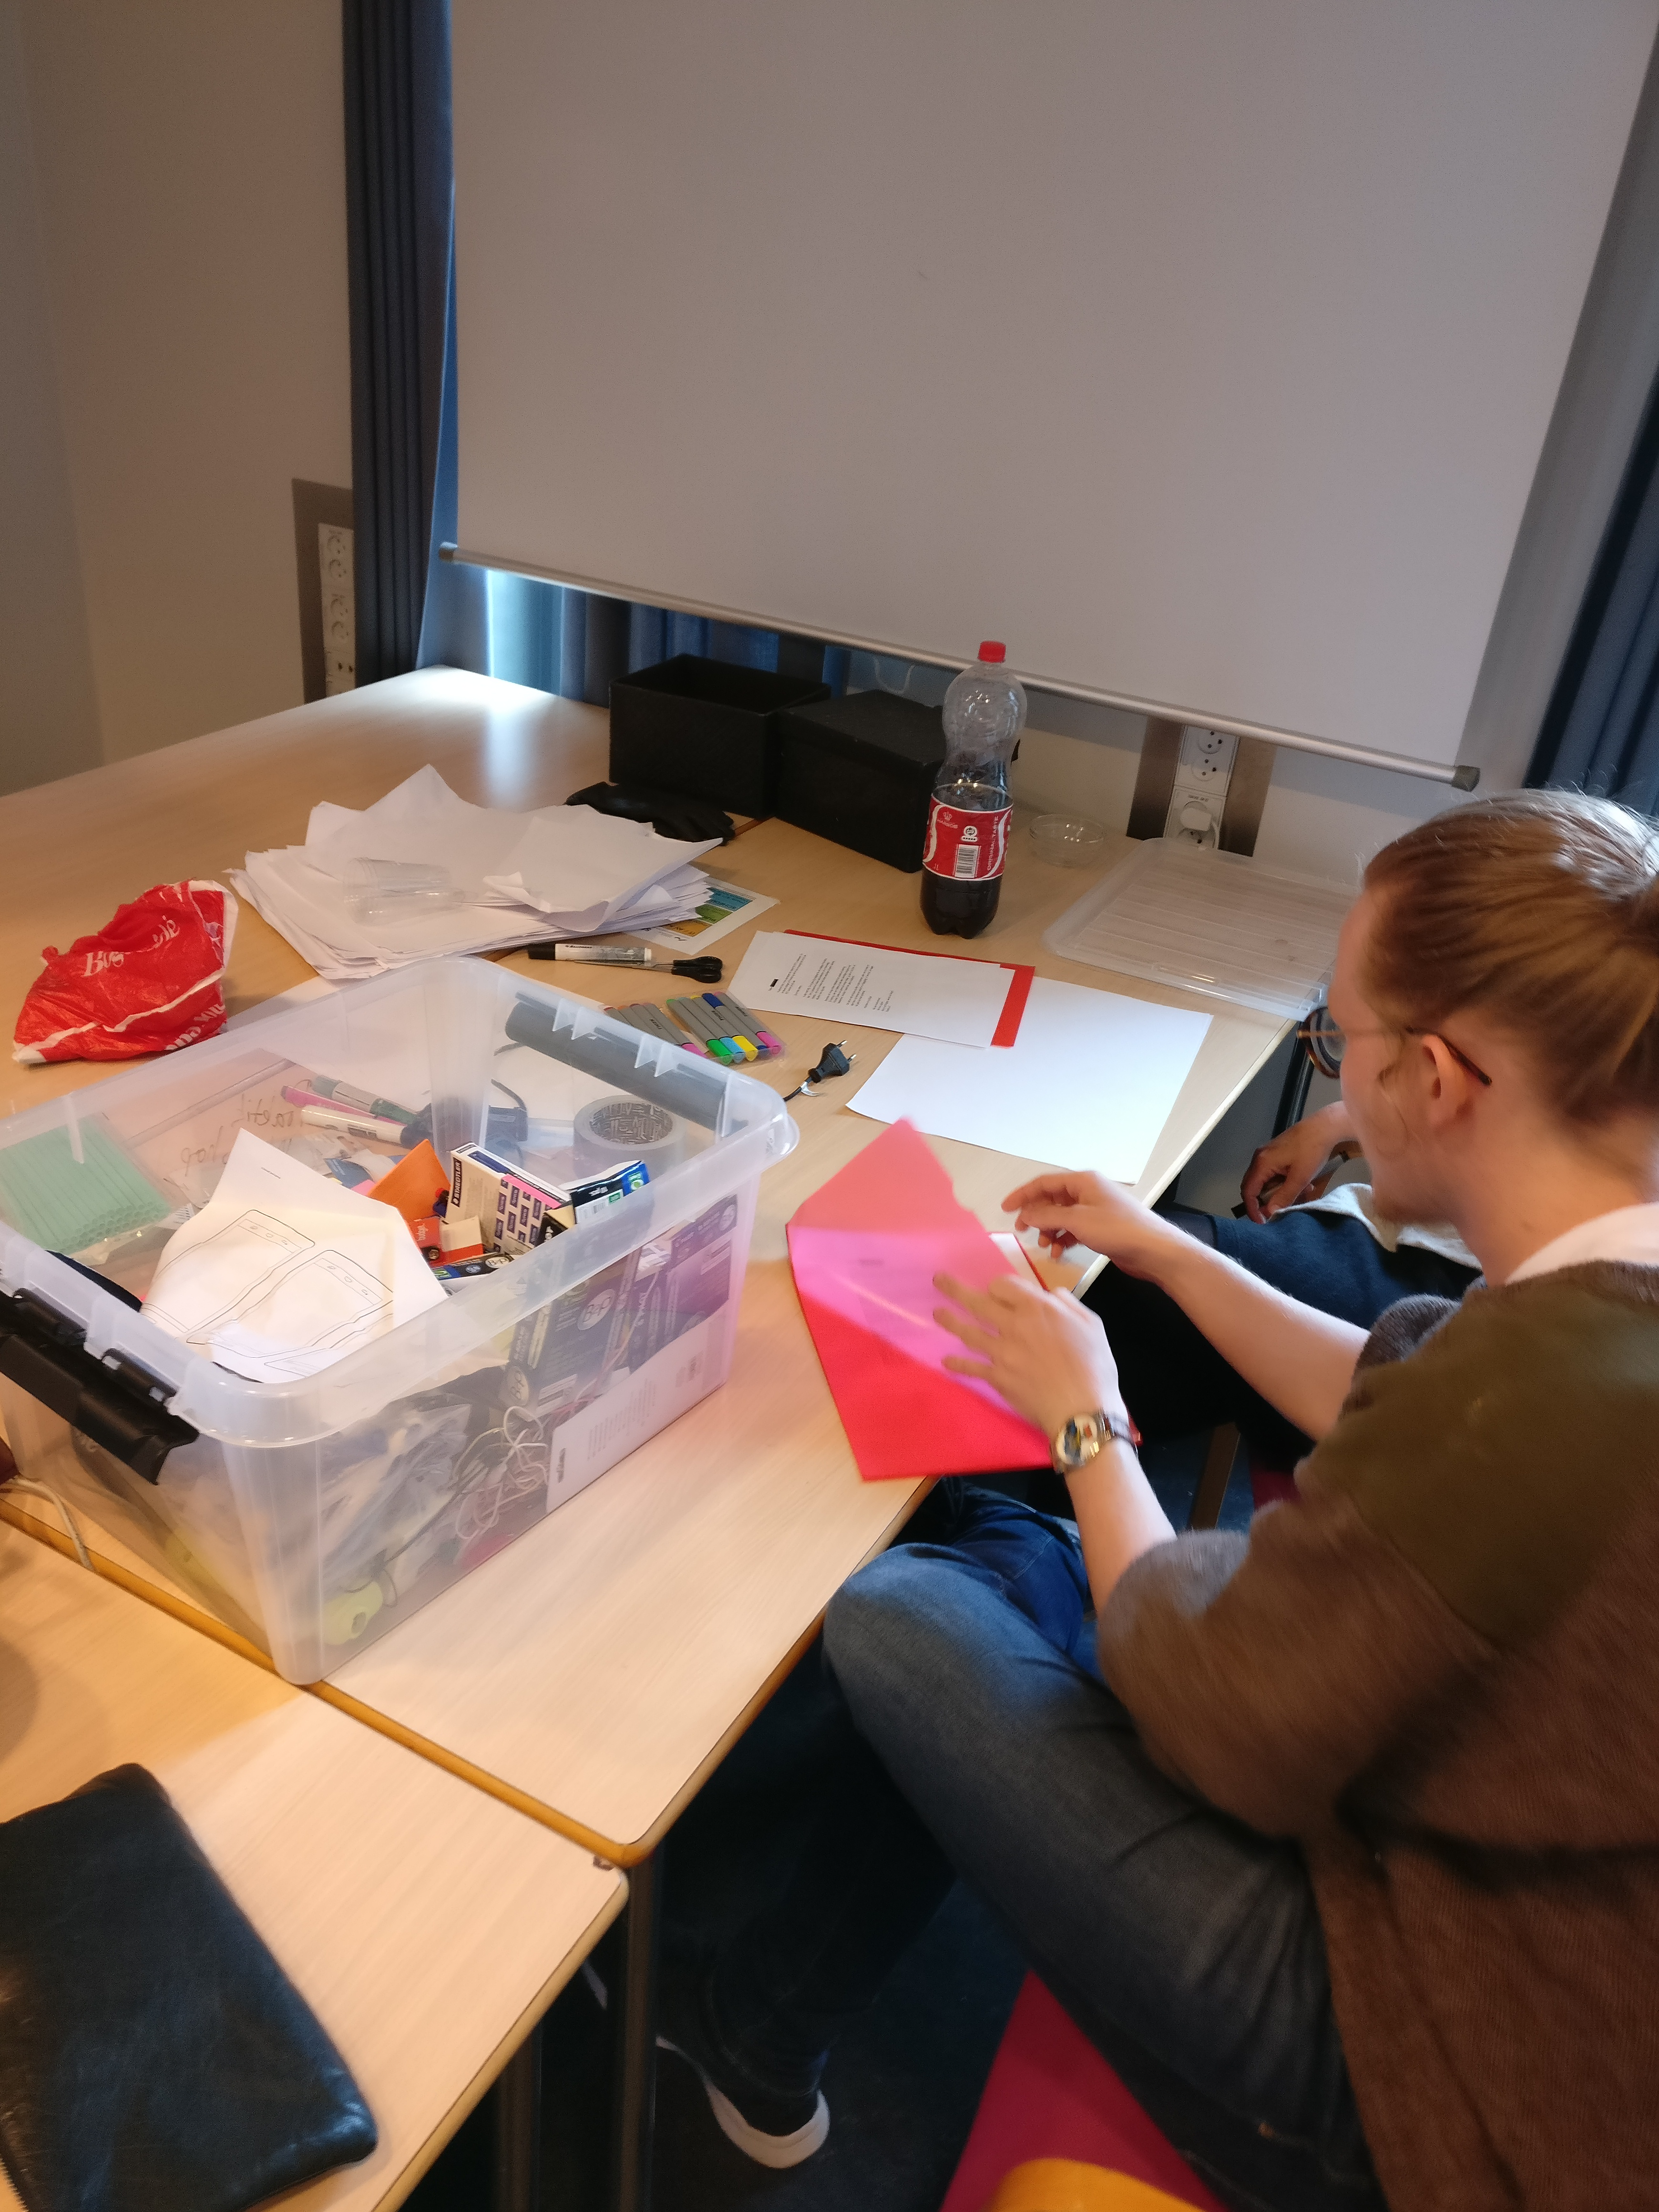
\includegraphics[width=.8\linewidth]{Pictures/FI1}
    \caption{1}
  \label{fig:sfig1}
\end{subfigure}%
\begin{subfigure}{.5\textwidth}
  \centering
  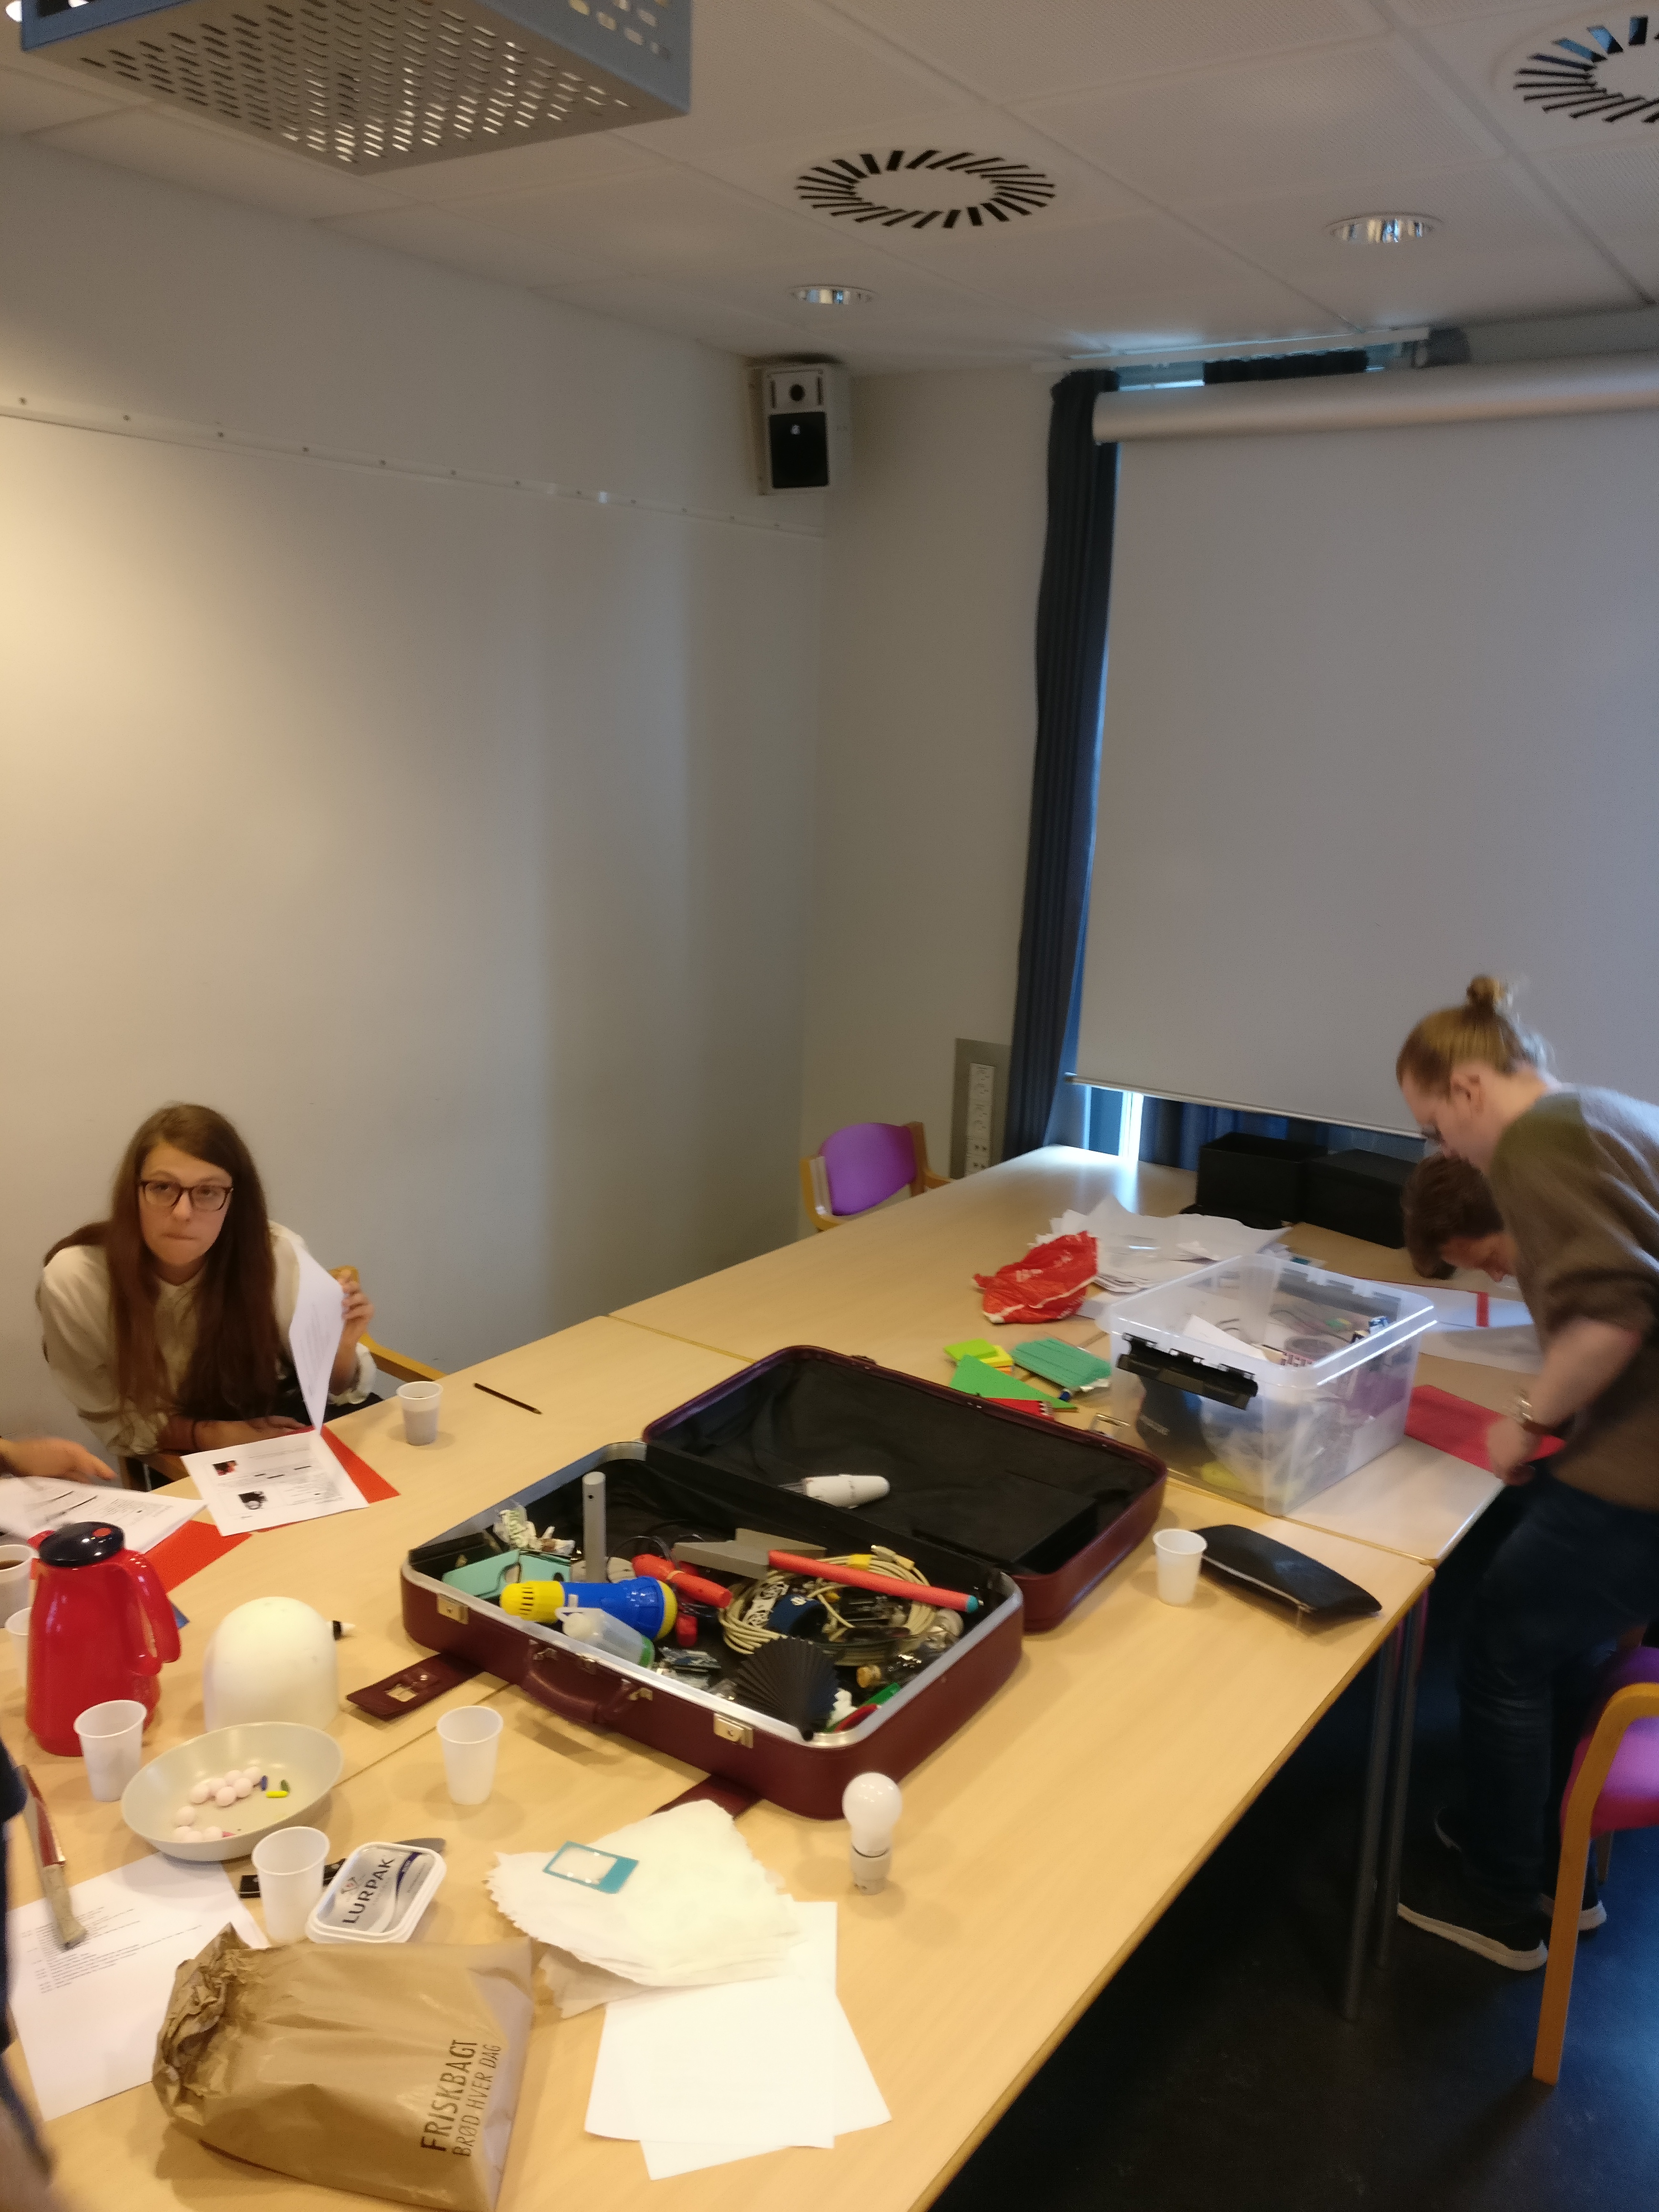
\includegraphics[width=.8\linewidth]{Pictures/FI2}
    \caption{2}
  \label{fig:sfig1}
\end{subfigure}
\begin{subfigure}{.5\textwidth}
  \centering
  \includegraphics[width=.8\linewidth]{Pictures/FI3}
    \caption{3}
  \label{fig:sfig2}
\end{subfigure}
\begin{subfigure}{.5\textwidth}
  \centering
  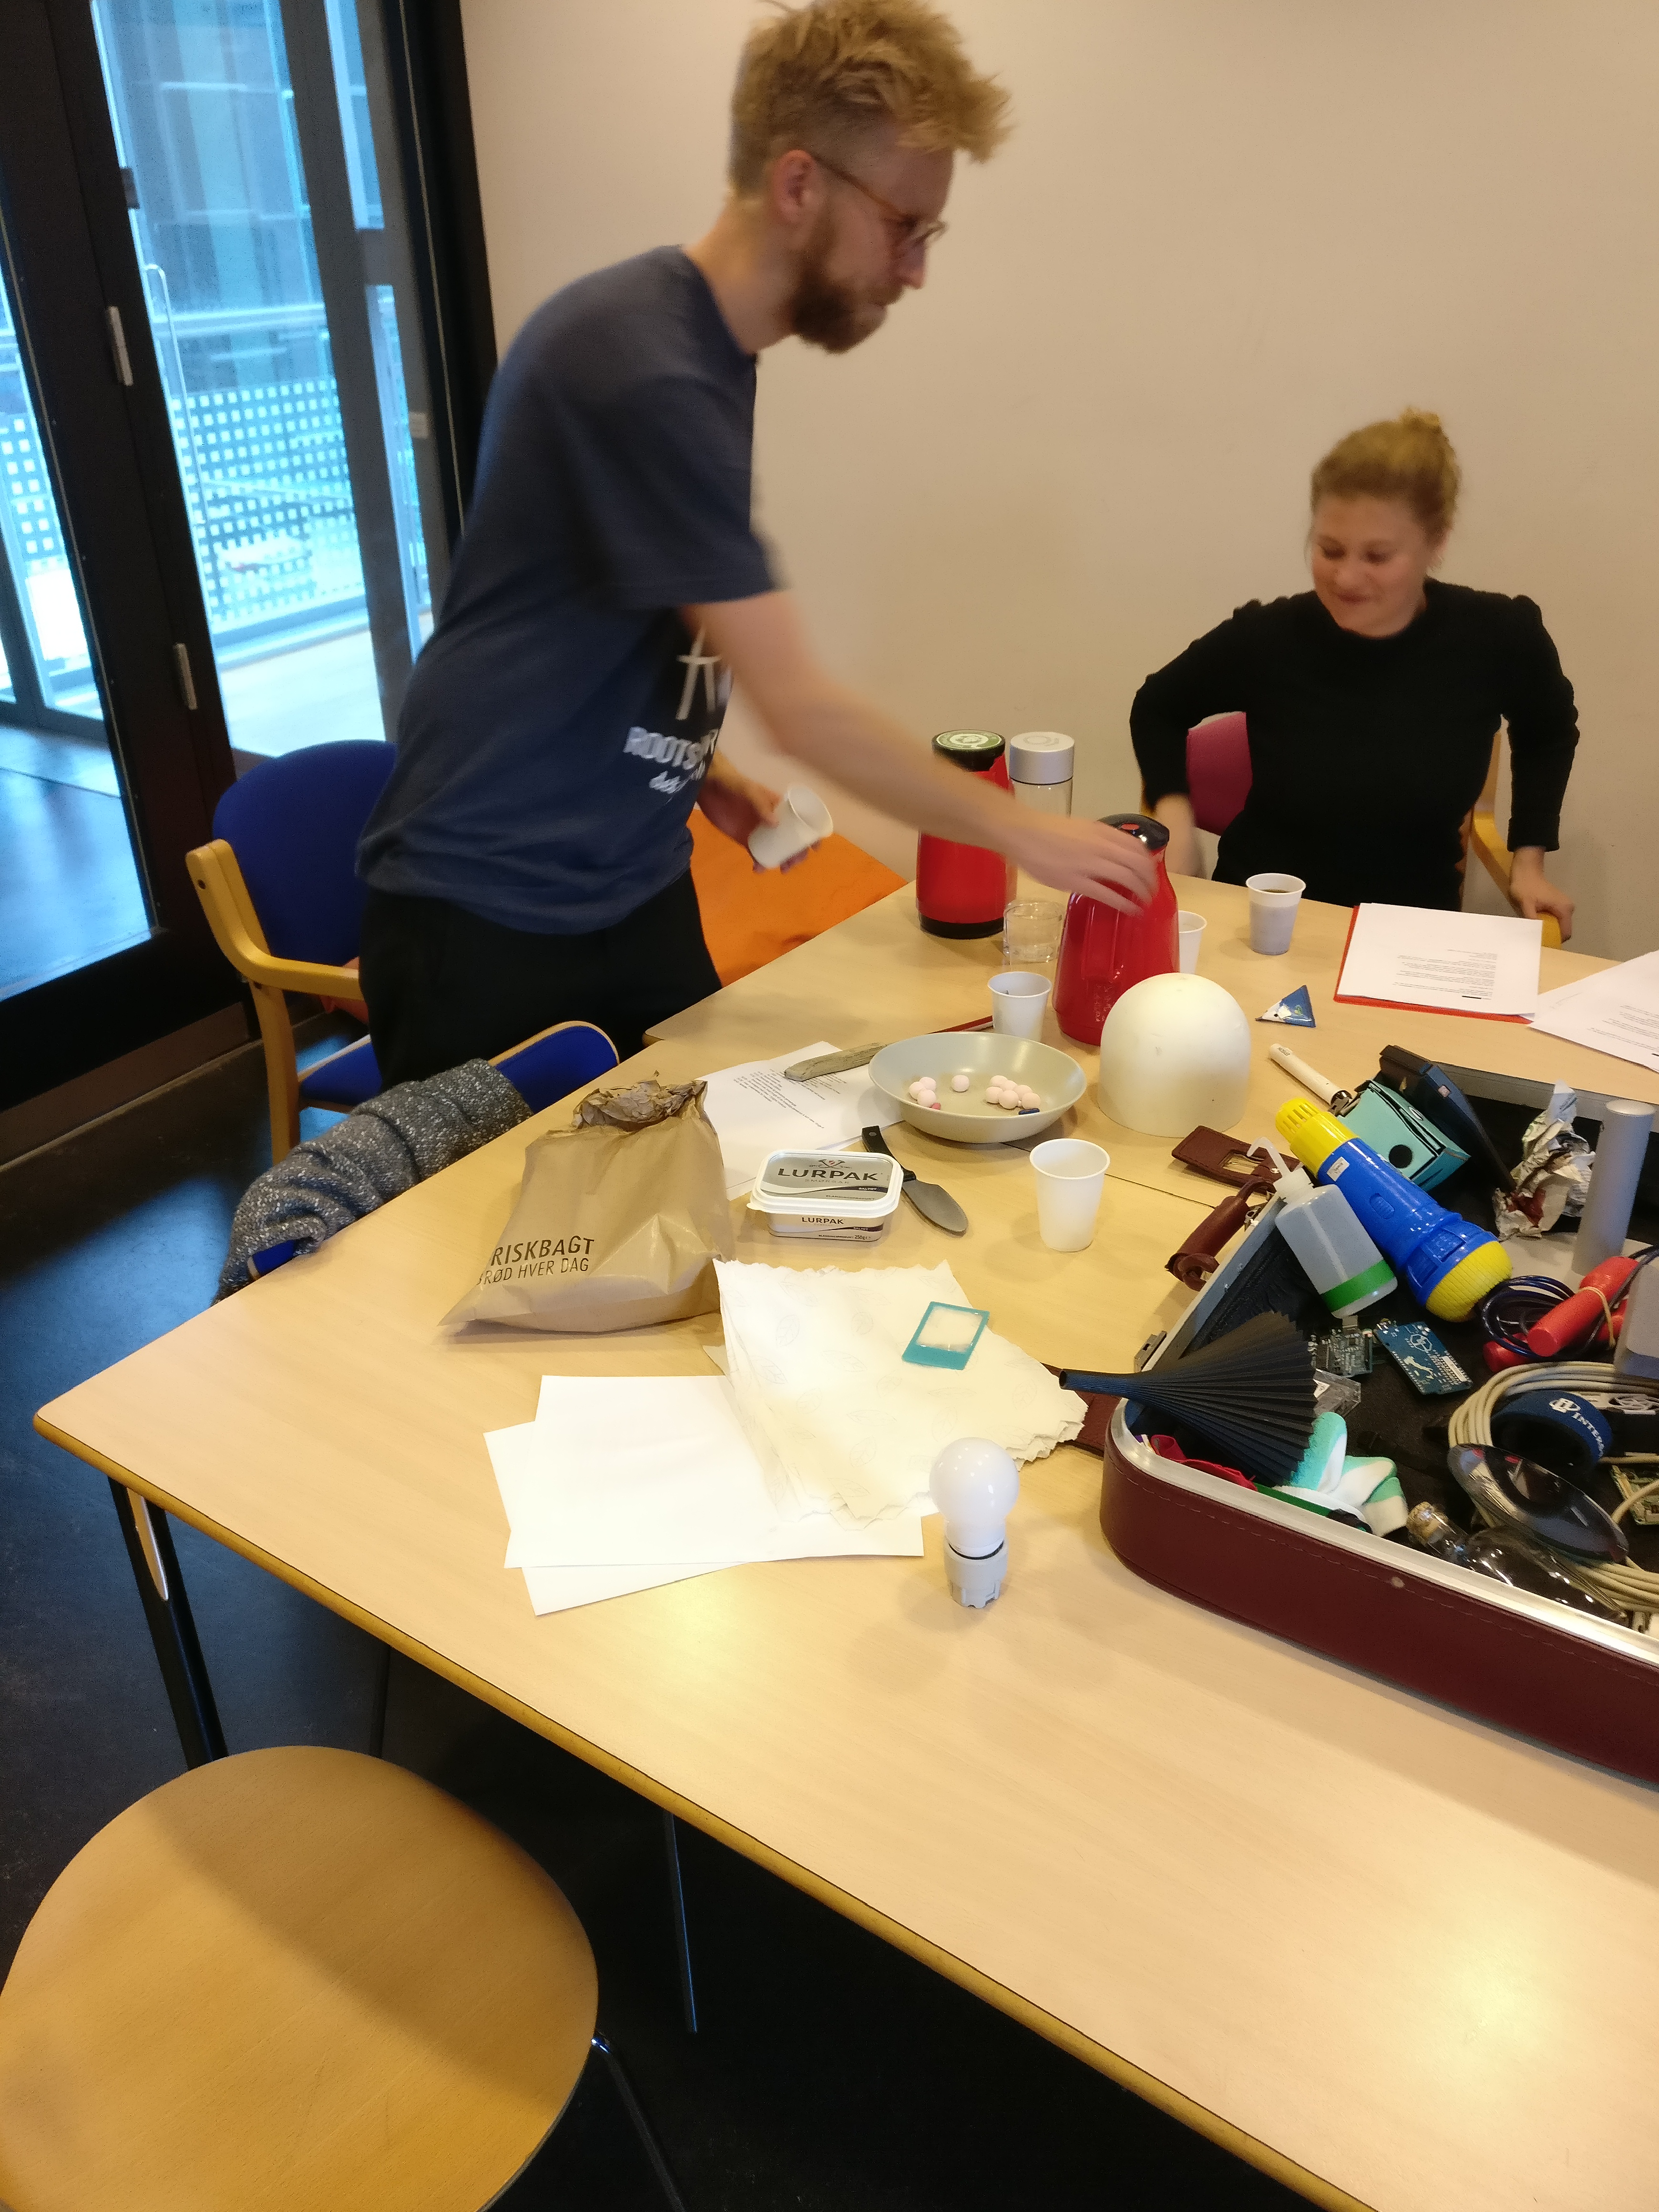
\includegraphics[width=.8\linewidth]{Pictures/FI4}
  \caption{4}
  \label{fig:sfig1}
\end{subfigure}%
\caption{Fictional Inquiry workshop, hvor deltagerne er blevet mistænkt på baggrund af Big Data}
\label{fig:fictional}
\end{figure}

Hvordan de ville løse opgaven var frit for. Vi havde fyldt en "spionkuffert" op med genstande, der alle i narrativet kunne bruges til at skabe, slette eller manipulere data. Først gennemgik vi i fællesskab genstandende. Dernæst blev deltagerne delt ind i to grupper og sat i gang. Vi deltog selv i arbejdet i de to grupper på lige fod med de øvrige deltager og sørgede for ikke at dominere processen, men i stedet agere fascilitatorer.

Grupperne udarbejdede en fire prototyper baseret på forskellige ideer om, hvordan PET kunne omgås. Der var især to aspekter, som gik igen i de forskellige prototyper. Først og fremmest var kontrol af data et emne. Alle fire prototyper indebar en skærpet kontrol af den data, der blev opsamlet om en. Dette var dog manifesteret for forskellig vis. I en prototype kunne man åbne en forbindelse til "skyen" og fysisk enten slette eller manipulere sin data ved hjælp af en speciel tang. 

Et andet central emne i workshoppen var \textit{bedre} data. I en prototype kunne man i en personlig databank optage og gemme sine tanker og minder. På denne måde kunne man lagre data som PET og andre overvågere ellers aldrig ville kunne få adgang til. I en anden prototype optog man kontinuerligt data af forskellig art og gemte det på et kassette bånd. Med denne personlige dataopsamler kunne man altså optage data uanset, hvor man var, eller hvad man lavede. Tanken bag begge disse prototyper lavet af to forskellige grupper var, at hvis man kunne optage data, der var \textit{bedre}, altså mere privat eller sværere at få fat på, kunne man konkurrere med det system, der overvågede en.

\subsection*{Den anden iteration}
Narrativet i det udførte Fictional Inquiry viste sig en effektiv måde at få deltagerne til at forholde sig kritisk til brugen af Big Data. Selvom prototyperne, der kom frem under workshoppen er designet ind i en fremskrevet verden, så vi alligevel elementer, der kunne tilbagebringes til en nutidig kontekst uden at miste deres evne til at skabe refleksion. Derfor kombineredes de to centrale elementer fra workshoppen, nemlig ejerskabet og kontrollen over ens egen data samt evnen til at optage og gemme kvalificeret data om en selv, med elementer fra TOTEM konceptet. Fra TOTEM fandt vi inspiration i det stærke fællesskab, produktet skaber. Det enkelte individ står stærkere i kraft af, at fællesskabet og datamængden vokser. I figur~\ref{fig:abakse} vises den serielle proces fra den første workshop frem til dataman.

Derpå designede vi Dataman.

\begin{figure}
    \centering
    \includegraphics[width = \textwidth]{Pictures/abakse.png}
    \caption{Den serielle proces fra den første workshop frem til dataman}
    \label{fig:abakse}
\end{figure}

%Lave a-b spektre med de forskellige produkter

\begin{comment}



\end{comment}
